\paragraph{Method.} The serving experiments replay one fixed sequence of 200 synthetic analyst
requests (\texttt{data/requests/requests\_seed42.jsonl}, seed 42):
\begin{itemize}
\item Poisson arrivals at unit rate, scaled to the target rate, so every run sees the same jobs;
\item 60\,\% optical jobs on the D3 mosaic with square AOIs of 0.5, 1 or 2\,km;
\item 40\,\% SAR or fused jobs on the demo band with 0.5 or 1\,km AOIs;
\item 20\,\% high priority (priority 5 against 0).
\end{itemize}
The replay is open-loop: each request is sent at its scheduled time, whatever the state of
earlier ones. A closed-loop generator such as Locust waits for each user's previous
request, which hides queueing delay at high load. Latency is taken from the database
timestamps, from submission to result ready.

Between runs, the worker is recreated with the arm's scheduling and the job tables are
emptied. Load is given in multiples of a capacity measured with a burst of 24 simultaneous
requests: 0.091\,jobs/s (Decision D8). The stack runs on the laptop: GTX 1650, WSL limited
to 4.8\,GB of RAM, worker container limited to 4\,GB. AOIs of 5\,km are left out for memory.

\paragraph{E4: latency against offered load.}
Latency stays flat up to 3$\times$ the burst capacity (0.27 jobs/s): p50 is 4--6\,s and
p95 is 8--14\,s, while throughput grows from 2 to 23\,km$^2$/min. At 4$\times$ the queue
builds (p50 95\,s, p95 266\,s) while throughput levels off at 22\,km$^2$/min, so the
saturation point lies between 0.27 and 0.37 jobs/s (Fig.~\ref{fig:load},
Table~\ref{tab:load}). The burst understates the sustainable rate: 24 jobs arriving at
once keep two jobs in flight all the time and fill the 4\,GB of GPU memory (peak
4056\,MiB), whereas steady arrivals rarely overlap below the knee. The GPU stays at
4--35\,\% utilisation throughout, because reading and normalising tiles (CPU) take most of
each job's time.

\paragraph{E2: batching policy at 3$\times$.}
Batching tiles across jobs is what keeps the service out of saturation. Per-job batches
(the baseline) reach 14.6\,km$^2$/min with p50 202\,s. Cross-job batches with a 10 or
25\,ms hold-back reach 18.4--19.2\,km$^2$/min (+30\,\%) with p50 84--89\,s
(2.3$\times$ lower). A 50\,ms hold-back is as bad as per-job batching (14.3\,km$^2$/min,
p50 199\,s): the GPU waits for batches to fill while jobs queue, and its utilisation drops
to 40\,\%.

\paragraph{E3: queue policy.}
The queue ranks jobs by $\text{priority} + a\cdot t_{\text{wait}}$.
\begin{itemize}
\item \textbf{At 4$\times$,} priority with ageing $a = 0.1$/s cuts the p95 latency of
high-priority jobs from 673\,s (FIFO) to 323\,s ($-52$\,\%) and their p50 from 484\,s to
184\,s. Normal jobs are no worse off: their p95 is 550\,s, against 704\,s under FIFO.
\item \textbf{At 3$\times$} that policy gives no gain (high-priority p95 125\,s for
both). With $a = 0.1$/s, a waiting normal job outranks a newly arrived high-priority job
after $5/0.1 = 50$\,s, and queue waits at this load exceed that, so the order is close to
FIFO. Ageing trades the responsiveness of high-priority work against a starvation bound.
\item \textbf{Slower ageing} ($a = 0.01$/s, so priority holds for 500\,s) gives the
clearest result. The p95 latency of high-priority jobs falls to 40\,s at 3$\times$
($-68$\,\% against FIFO) and to 74\,s at 4$\times$ ($-89$\,\%), with p50 of 16 and
33\,s. Normal jobs pay for it, but within the same order as FIFO: p95 158\,s against
109\,s at 3$\times$, and 551\,s against 704\,s at 4$\times$. Throughput stays close to
FIFO (17.6 against 18.3\,km$^2$/min at 3$\times$, 12.6 against 10.7 at 4$\times$),
because the policy only reorders the same work.
\end{itemize}

\paragraph{Caveats.} The laptop warmed from 72 to 89\,$^\circ$C over the session, and
per-job CPU time doubled with it. Comparisons are therefore made within an experiment,
whose arms ran back to back, and not across experiments. For example, the 3$\times$ point
of E4 ran cooler than the E2 arms at the same load. The Docker VM clock occasionally jumped
by 5\,h\,30\,min (UTC against IST). Those timestamps are corrected by the jump and
counted. After correction, every run's makespan agrees with its client-side wall time to
within 4\,\%.

\begin{figure}[t]
\centering
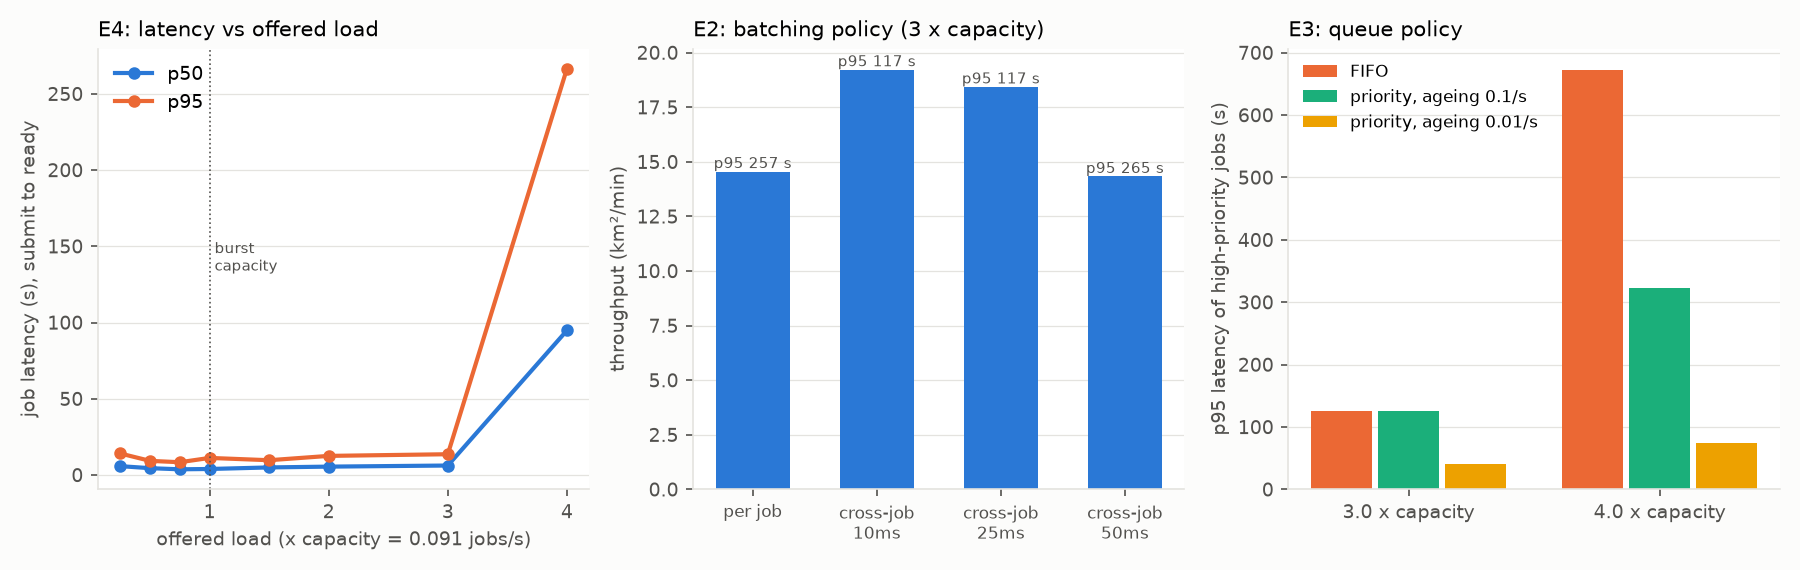
\includegraphics[width=\linewidth]{e_load.png}
\caption{Serving experiments on the laptop stack. Left: E4 job latency (p50, p95) against
offered load. Middle: E2 throughput by batching policy at 3$\times$ (labels: p95).
Right: E3 p95 latency of high-priority jobs by queue policy.}
\label{fig:load}
\end{figure}

\begin{table}[t]
\centering\small
\begin{tabular}{llrrrrrr}
\toprule
Exp. & Arm & Load & p50 (s) & p95 (s) & High-prio p95 (s) & km$^2$/min & GPU \\
\midrule
cap. & burst of 24 & burst & 125.6 & 235.4 & 39.6 & 8.6 & 63\,\% \\
E4 & cross-job 25 ms, priority & 0.25$\times$ & 5.8 & 14.1 & 7.9 & 2.0 & 4\,\% \\
E4 & cross-job 25 ms, priority & 0.50$\times$ & 4.5 & 9.2 & 8.6 & 3.9 & 5\,\% \\
E4 & cross-job 25 ms, priority & 0.75$\times$ & 3.7 & 8.3 & 6.5 & 7.6 & 10\,\% \\
E4 & cross-job 25 ms, priority & 1.00$\times$ & 3.9 & 11.2 & 6.3 & 9.6 & 12\,\% \\
E4 & cross-job 25 ms, priority & 1.50$\times$ & 4.9 & 9.7 & 10.9 & 15.0 & 19\,\% \\
E4 & cross-job 25 ms, priority & 2.00$\times$ & 5.5 & 12.5 & 12.2 & 17.0 & 22\,\% \\
E4 & cross-job 25 ms, priority & 3.00$\times$ & 6.2 & 13.6 & 14.0 & 23.4 & 34\,\% \\
E4 & cross-job 25 ms, priority & 4.00$\times$ & 94.8 & 266.4 & 115.0 & 22.2 & 35\,\% \\
\midrule
E2 & per job 0ms & 3.00$\times$ & 201.8 & 256.7 & 201.0 & 14.6 & 60\,\% \\
E2 & cross job 10ms & 3.00$\times$ & 83.9 & 117.4 & 69.9 & 19.2 & 53\,\% \\
E2 & cross job 25ms & 3.00$\times$ & 89.3 & 116.7 & 65.7 & 18.4 & 61\,\% \\
E2 & cross job 50ms & 3.00$\times$ & 198.7 & 264.6 & 209.7 & 14.3 & 40\,\% \\
\midrule
E3 & fifo & 3.00$\times$ & 45.7 & 113.1 & 125.8 & 18.3 & 34\,\% \\
E3 & priority & 3.00$\times$ & 138.1 & 168.4 & 125.0 & 17.0 & 30\,\% \\
E3 & fifo & 4.00$\times$ & 449.2 & 703.4 & 672.7 & 10.7 & 55\,\% \\
E3 & priority & 4.00$\times$ & 271.9 & 540.2 & 322.9 & 12.7 & 41\,\% \\
E3 & priority ageing0.01 & 3.00$\times$ & 34.7 & 155.2 & 40.0 & 17.6 & 37\,\% \\
E3 & priority ageing0.01 & 4.00$\times$ & 379.1 & 541.5 & 74.2 & 12.6 & 41\,\% \\
\bottomrule
\end{tabular}
\caption{Serving runs on the laptop stack (re-summarised from the raw job records;
load in multiples of the burst capacity, 0.091 jobs/s).}
\label{tab:load}
\end{table}

